\documentclass[12pt]{article}
%\usepackage{bookman}
\usepackage{/home/sci/weiliu/haldefs}
\usepackage{graphicx}
\usepackage{url}
\usepackage{textcomp}
\usepackage{enumitem}
\usepackage{subfig}
\usepackage{hyperref}
%\usepackage{/home/sci/weiliu/packages/breakurl/breakurl}
\usepackage{amsmath}
\usepackage{verbatim}
\usepackage{natbib}
\usepackage{algorithmic}
\usepackage{algorithm}
\usepackage{color}
\usepackage{mdwlist}

\hypersetup{
  % bookmarks=true,         % show bookmarks bar?
    unicode=false,          % non-Latin characters in Acrobat’s bookmarks
    pdftoolbar=true,        % show Acrobat’s toolbar?
    pdfmenubar=true,        % show Acrobat’s menu?
    pdffitwindow=false,     % window fit to page when opened
    pdfstartview={FitH},    % fits the width of the page to the window
    pdftitle={Reading notes},
    pdfauthor={Wei Liu},     % author
    pdfsubject={Reading notes},   % subject of the document
    pdfcreator={Wei Liu},   % creator of the document
    pdfproducer={Producer}, % producer of the document
    pdfkeywords={reading, papers, functional MRI, connectivity}, % list of keywords
    pdfnewwindow=true,      % links in new window
    colorlinks= true,       % false: boxed links; true: colored links
    linkcolor=blue,          % color of internal links
    citecolor=blue,        % color of links to bibliography
    filecolor=magenta,      % color of file links
    urlcolor=cyan           % color of external links
}


\setlength{\oddsidemargin}{0 in}
\setlength{\evensidemargin}{0 in}
\setlength{\topmargin}{-0.6 in}
\setlength{\textwidth}{6.5 in}
\setlength{\textheight}{9 in}
\setlength{\headsep}{0.5 in}
\setlength{\parindent}{0 in}
\setlength{\parskip}{0.1 in}



\begin{document}
\title{Reading notes}
\author{Wei Liu}
\maketitle
%% \tableofcontents

This is a summary of the readings of the recent functional connectivity papers. 

\textbf{dynamic connectivity: } It looks like people are begining to study the
dynamic property of the connectivity \citep{deco2010emerging}. The conventional
brain connectivity analysis assume that the connections between regions are
static and do not change with time. \cite{zalesky2011relationship} test the
variation of the fMRI time series by splitting the time series into two part,
and use paired t-test to test any difference between two halves with respect to
the various statistical measures, including variance, maximum and minimum
amplitude, and did not identify significant difference. This suggest there is no
long-term variation on the time series. But this is not sufficient to suggest
that the functional network is static. The connectivity between any regions can
change over time. Modeling the dynamics of the connectivity will help to
understand the brain network. If we use graph to model brain network, we can use
the rich theory in the dynamics of the graph \citep{mortveit2008introduction} to
model the dynamics of the brain network. \cite{deco2010emerging} reviewed three
typical methods for modeling the network dynamics.


\section{Sparsity of Brain Network}
Theare are a few reasons that we should explore the sparse concept of graphical
model to fMRI.
\begin{itemize}
  \item \textbf{Consistence with neurophysiology} The coefficients computed the
    regression with sparcity method corresponds to the partial correlation after
    removing the influence of all other nodes in the graph. This amounts to the
    direct connection between two regions. The regular correlation matrix have a
    marginal interpretation. The inverse covariance matrix of the multi-variate
    Gaussian gives a \emph{conditional} interpretation. The zeros in the
    precision matrix means conditional independence given all other nodes, and
    the coefficients means partial covariance (or partial correlation, after
    normalization of the the data).

    Any two regions of the human may have some degree of correlation marginally,
    due to the possible connections to other nodes. The partial correlation
    answer the questions like what is the direct link between two regions. This
    can also be explained with diffusion tensor imaging where fiber tracts
    either directly or indirectly connect two white matter regions.

  \item \textbf{Rich method for optimization}
  \item \textbf{Network analysis as postprocessing}
  \item \textbf{Possibility to parallelize} The graphical Lasso problem can be
    seen as $P$ independent linear regression problem, which can be
    parallelized.
\end{itemize}

\section{April 2 - 9}
The functional network is said to be orgainized in a hierarichical way. We can
explore this.

Markov Random field can be used in functional connectivity of fMRI data and
represent the statistical dependency of spatial adjacent variables. The
representation can be either in voxel level or in a higher level where objects
or regions of interest are variables. The topology or structure of the graph
used by MRFs can be known as regular lattice, or it can be learned from the
data. The model as a prior information, helps the statistical inference of the
connectivity.

\section{April 9 - 16}
Need to test synthetic data for parameter estimation. Find a scenario where the
parameters can be decently estimated. We need a good validation method for this
hierarchical MRF method.

Also need to revise the thesis claim. And for the dynamical network, draft a summary of the readings. 

\citet{honey2007network} studies the dynamics of functional network on a single
subject. It is helpful if we can build a model that can use information from
multiple subjects. in \cite{honey2007network}, the structure connectivity matrix
is first computed, and neural dynamical potential signal is \emph{simulated} by
some models. The neural potential has high sampling rate. The functional
connectivity is computed from this simulated time course signal at different
temporal scale. BOLD signal is also \emph{simulated} from the neural potential
signal by the \emph{balloon} model. It seems the simulated BOLD signal has
course spatial resolution compared the neural potential signal, i.e., BOLD is
simulated per region. The conclusion is that functional connectivity estimated
from the whole neural potential signals are more consistent with structural
network, while the network estimated from a segment of neural signals have more
transient network patterns.

My comments: For the study of fMRI, we do not have to assume a model for neural
potential signal and simulate it. We can just assume a dynamic for BOLD
signal. The model should take account multiple subjects. We should model the
common property among all the subjects. For example, although different subjects
may not in the same state at same time point on same ROI, they may share
probability of transiting from one state to the next. Subjects must share
something.

To model the dynamics of the network, we can either explicitly model the time
delay due to the transmission of the neural signal in the fibers, or we can
choose not model this time delay. \cite{honey2007network} does not model it. We
probably should not model it either, because the low temporal resolution of BOLD
signal. The time delay, compared to the TR of BOLD, can be ignored.

\cite{ghosh2008noise} is the second paper that \citet{deco2010emerging}
reviewed. In \citeauthor{ghosh2008noise}, the low level neural singal is also
simulated similar to \citeauthor{honey2007network}, and BOLD signal is computed
from these simulated signals. The difference from \citeauthor{honey2007network}
is they add time delay between the regions, and the delay is proportional to the
distance between the regions.

If we have a dynamical model for BOLD signal, how could we simulated it to see
the simulated BOLD signal look like the real data? Dynamical Gaussian Markov
Random Field???

In \cite{yeo2011organization}, 7 and 17 functional network is estimated by
clustering approach. This functioal atlas is used in a review of ADHD
\citep{castellanos2011large}. From \citeauthor{castellanos2011large}, DMN is has
less anti-correlation for ADHD patients, since the strong anti-correlation is
believed to related to the better behavioral performance.

Another interesting thing to do is building a spatial-temporal model of fMRI
data. The model will depict the spatial dependency, as well as the temporal
correlation of the BOLD signal. This model can be used to estimate and remove
noise. Such a model is related to the MRF because spatially it would be a MRF,
and temporal domain the image at time point $t$ will depend on the image at
$t-1$.

\section{April 23 - 30}
What we have been done so far is far from being a jounarl paper. 

The advantage of variational inference: 1) Able to estimate number of components
K. 2) Use indicator vector notation instead of scalar variable for hidden
variables. 3) Introduce Dirichlet distribution for the mixing coefficients
pi. 4) Less memory usage. 5) Less running time. 6) Possible for full Bayesian
analysis.

The advantage of using \textsf{lemon} graph library for rewriting the code: 1)
Graph structure separate from data. 2) Easier to change graph structure without
chaging other code. 3) Ease to change MRF neighborhood structure, say, from 6
neighbors to 26 neighbors.

The Dirichlet prior on mixing coefficient Pi is different from the MRF on hidden variable z.

\section{April 30 - May 6}
\subsection{Consistency test}
This test aims to see the consistency of the joint log likelihood function $p(x,y)$ over the number of MC samples. 
\begin{figure}
  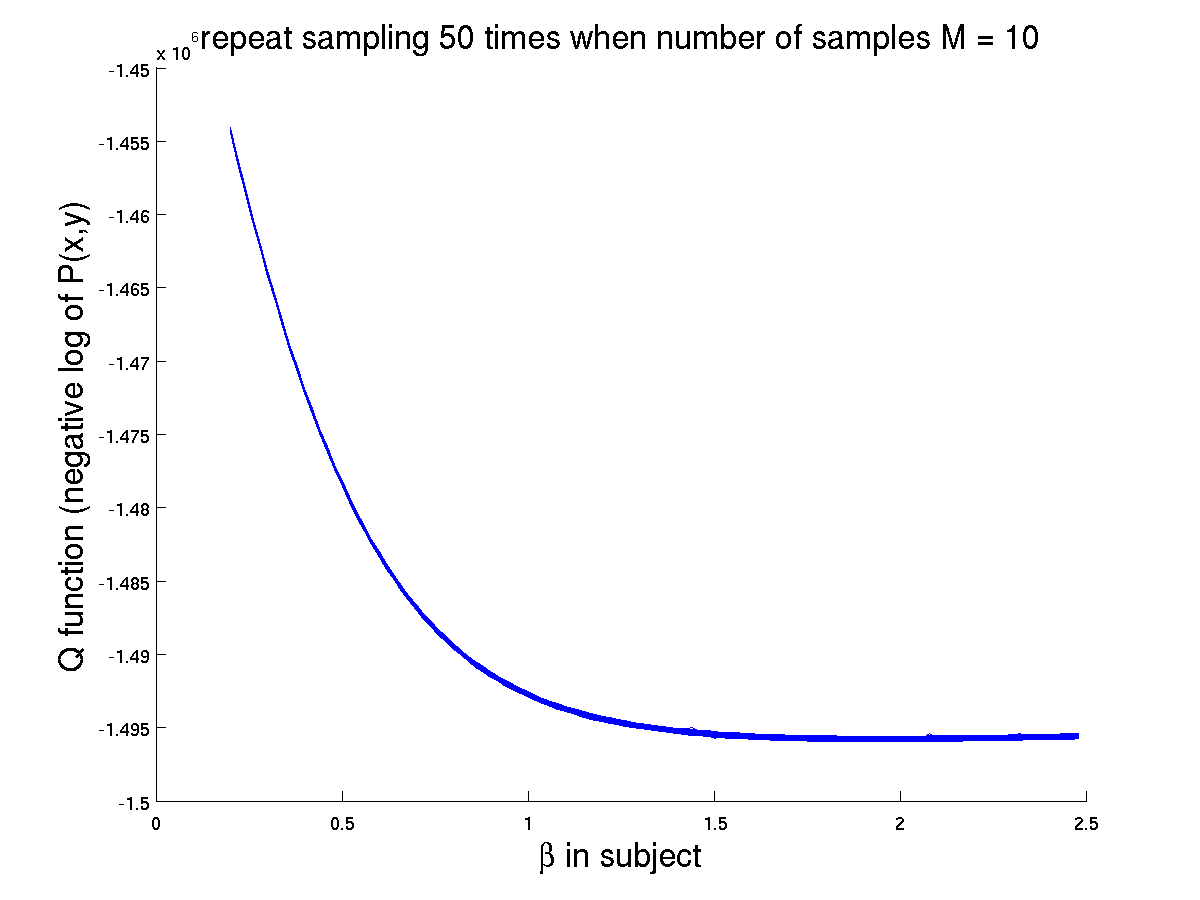
\includegraphics[width=0.45\textwidth]{figures/n10}
  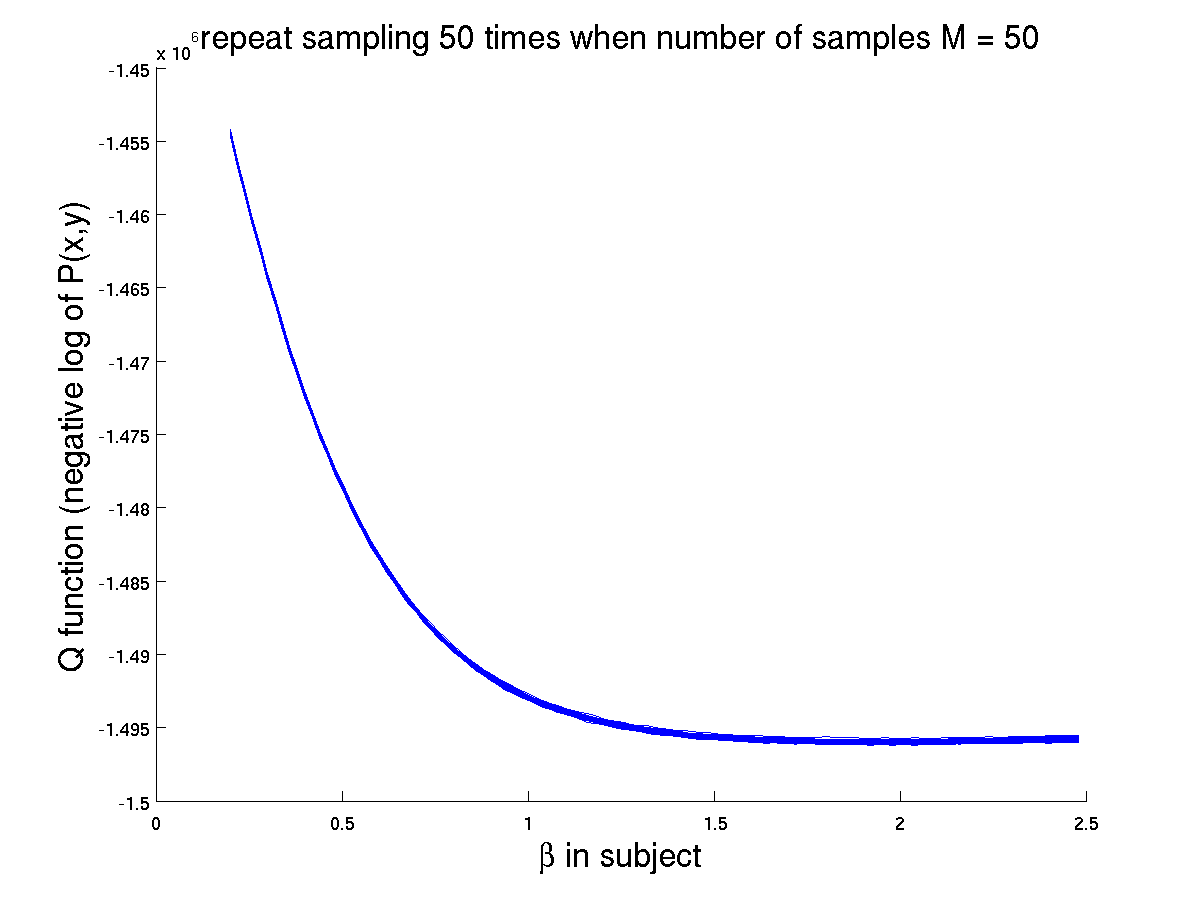
\includegraphics[width=0.45\textwidth]{figures/n50}\\
  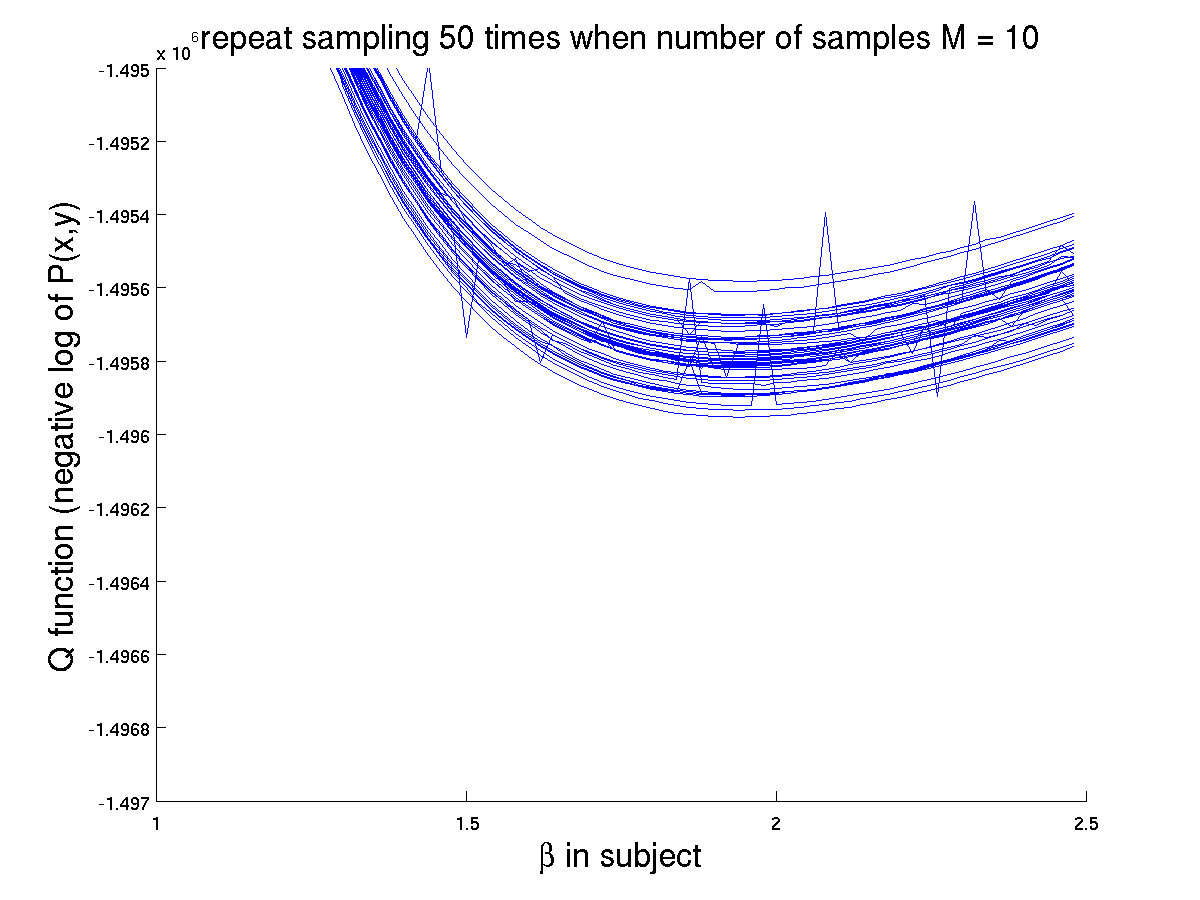
\includegraphics[width=0.45\textwidth]{figures/n10_zoom}
  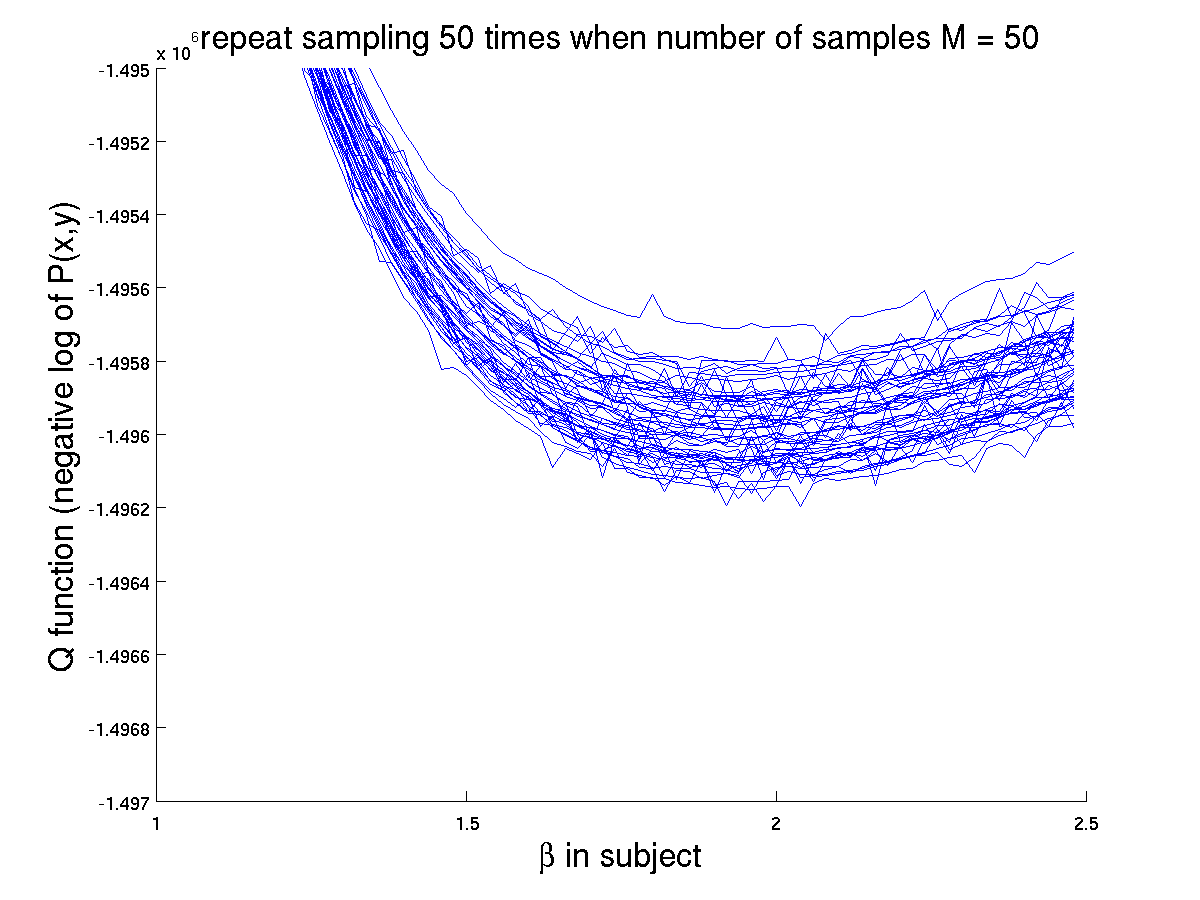
\includegraphics[width=0.45\textwidth]{figures/n50_zoom}
\end{figure}
\subsection{Swendsen-Wang}
First I will explain how Swendsen-Wang sampling works on a simple Ising or Potts model. Define the Potts mode as
\begin{align*}
  f(x) &= \frac{1}{Z}\exp \{H(x)\}, \quad H(x) = \sum_{i<j} \beta \Ind_{(x_i = x_j)}.
\end{align*}
This is a slightly different definition with our previous definition of Potts model, but they both prefer smoothed labels between spatial neighbors when $\beta > 0$. Now to generate a sample from $f(x)$, we introduce a auxiliary random variable $y_{ij}, i \le j$. Conditioned on $x$, the $y_{ij}$ are independent. Each $y_{ij}$ is uniformly distribution on the interval $[0, a_{ij}]$, with $a_{ij} = \exp(\beta\Ind_{(x_i = x_j} ) \leq 1$. So the conditional pdf of $y = \{y_{ij}\}$ given $x$ is
\begin{equation*}
  f(y|x) = \prod_{i\le j}\frac{\Ind_{(y_{ij} \leq a_{ij})}}{a_{ij}} = \left (\prod_{i\le j}\Ind_{y_{ij} \leq a_{ij}} \right )\exp \{-H(x)\}
\end{equation*}
Due to this definition of $f(y|x)$, the joint pdf $p(x,y)$ is also uniformly distributed because of the cancellation of $H(x)$ and $-H(x)$.
\begin{align*}
  f(x,y) &= f(x) f(y|x) = \frac{1}{Z}\exp\{H(x)\} \cdot  \left (\prod_{i\le j}\Ind_{y_{ij} \leq a_{ij}} \right )\exp \{-H(x)\} \\
  & =  \frac{1}{Z} \prod_{i\le j}\Ind_{y_{ij} \leq a_{ij}} = \left \{
  \begin{array}{l l}
    \frac{1}{Z} & \quad \text{if $y_{ij} \leq a_{ij}, \forall i < j,$}\\
    0 & \quad \text{otherwise}\\
    \end{array} \right.
\end{align*}
More importantly, $p(x|Y) \prop f(x,y)$ is also uniformly distributed over the
set $\cA = \{x: y_{ij} \leq a_{ij}\}$. Now either $y_{ij} \in [0, 1]$ or $y_{ij}
\in (1, e^\beta]$. if $y_{ij} \leq 1$, it is impossible to tell if $x_i =
  x_j$. But if $y_{ij} > 1$, $a_{ij} $ must be greater than 1 to allow draw a
  uniform sample $y_{ij} > 1$ from $f(y_{ij} | x)$, and hence $x_i =
  x_j$. Therefore, The sites $i$ and $j$ for which $y_{ij} . 1$ can be gathered
  into clusters, and within each such cluster the $x$ must be same. And the
  value of $x$ is uniformly distributed. The $x_i$ and $x_j$ value for those
  $y_{ij} \leq 1$ are not constrained to be same and can be different.

Hence we can sample from $f(y|x)$ and $f(x|y)$. At last we discard $y$ and the
$x$ will be samples from marginal distribution $f(x)$. To simplify matters
further, note that instead of the exactly $y_{ij}$ it suffices to know only the
variables $u_{ij} = \Ind_{y_{ij} \leq 1}$. Given $x$, $u_{ij}\sim \Ber(1 -
e^{-\beta})$ if $x_i = x_j$, and $u_{ij} = 0$ otherwise. Hence we have the
Swendsen-Wang algorithm as: 1) Given $x_i$, generate $u_{ij} \sim \Ber(1 -
e^{-\beta})$ if $x_i = x_j$, and $u_{ij} = 0$ otherwise. 2) Given $\{u_{ij}\}$,
generate $x$ by clustering all the sites and choosing a label value for each
cluster independently and uniformly from $\{1,\dots, K\}$.


\subsection{Generalized Swendsen-Wang}
The generalized Swendsen-Wang by \cite{barbu2005generalizing} has a few things to note:
\begin{itemize}
\item It choose only one cluster to change label $x$ in each iteration, instead of sample all clusters.
\item It seems the posterior distribution used in their sampling only includes likelihood term (i.e. the data term), and not includes the smoothness prior. This need special attention. 
\end{itemize}

\section{May 14 -- May 21}
Since he SW algorithm takes longer time than regular Gibbs sampler, I used a
profiler to look into the call trace of valgrind tool, and found that: When
sampling on a single larger image (128x128x128, which amounts to 10 subjects
data of real fMRI), about half of the running time is spent on finding connect
component. Around 25\% time is used for generating random samples. About 11\% is
spent on the other operations on the graph such as access nodes and edges.

If we want to re-write the code in parallel, at most 50\% of the routine can be
optimized, and the connect component routine can not be parallelized easily,
since it is provided by the \textsf{lemon} library. We do need this library in
order to define a data structure for both graph nodes and edges. Even if we do
not use this library, and write our own connected component routine, it is not
straightforward how to optimize it in parallel, since the algorithm is
implmented with a breath-first-search algorithm.

Other issues: Critical temperature,  variance map.

\section{Aug 24 -- Aug 27}
I'm currently working on two things: 1) I think we may need a change on the
hierarchical model. We don't really need the MRF in group level, since the
subjects MRF can enforce the smoothness of group. There are advantages of this
simplification: a) we can define 1-of-K binary vector on subjects level, and
define a continuous variable on group. So the group naturally acts as a prior
probability, just as we tried to do some time ago. b) It would be possible to
define a Dirichlet prior on group, and we can probably even estimate the number
of clusters K. 2) If the sampling algorithm's issue is too difficult to solve,
there is no reason we can not try other optimization methods like Variational
Inference. The benefits are: a) Full Bayesian. b) faster. The solution would
still be a local optima, though. There are rich theory along this path, so we
don't worry about the lack of good methodology/theory.

OK this is not the right thing to do for now. 

Wednesday: Spent some time on MTGL graph library. Though the computation time is
not a issue if the algorithm works fine, it is an issue when in debugging
stage. The MTGL library is claim to have parallel algorithm than can use
multiple threads. After looking into it, I found this is not what I want. I just
need use the Lemon graph library and update each node with my own pthread
routine. I don't really need a parallel a parallel graph library. MTGL's
parallel implementation is on some specific algorithm, which I don't need except
in a Swendsen-Wang algorithm for connected component analysis.

So if I do need a graph library, Lemon is the choice so far. But to migrate the
current code to the Lemon graph is low priority compared to testing on new
datasets.

Thursday and Friday: Downloaded NYU's test-retest dataset and working on the
preprocessing scripts. The plan is to use fcon 1000's scripts which uses FSL and
AFNI tool. This scripts is similar to ADHD200's scripts but is more geenral.

\section{Apr 14: Model Selection: Alpha}
This section is for choosing the optimal $\alpha$ parameter of the hierarchical
MRF model. I will define $\alpha$ as part of the model, and choosing $\alpha$
turns into a model selection problem. The Bayesian method of model selection is
to compute the marginal data likelihood, given as
\begin{align*}
  P(D | \cM) = \int P(D|\theta) P(\theta|\cM)\, \textrm{d}\theta,
\end{align*}
with $D$ the data, and $\cM$ the model, and $\theta$ the set of parameters. In
our model, the hidden network labels also need to be integrated out in order to
compute the above marginal distribution. Besides, the data used to train the
model should be different with the data for testing. Define $x$ is the training
subjects' fMRI data, and $y$ the training subjects label (include both group map
$y_g$ and subject maps $y_{sub}$), and $x_t$, $y_t$ are the test subject's fMRI
and label map. We can use the posterior predictive distribution defined as
\begin{align}
  P(x_t | \cM, x) = \int P(x_t | y_t; \theta_t) P(y_t| \cM, x; \theta)\, \textrm{d} y_t.
  \label{eq:predis}
\end{align}
$\theta_t = \{\mu_t, \kappa_t, \beta_t\}$ is the parameter set for the test
subject, and $\theta = \{\mu, \kappa, \beta\}$ is the set of parameters for the
training subjects. The $\alpha$ parameter goes into the model $\cM$, and we
choose $\alpha$ with the largest distribution given above. To evaluate the above
distribution, we can use the MC integration by drawing samples of $y_t$ from
$P(y_t, \theta|\cM, x; \theta)$
\begin{align*}
  P(x_t | \cM, x) \approx \frac{1}{M}\sum_m P(x_t|y_t^m; \theta_t), \qquad y_t^m \sim P(y_t|\cM, x; \hat \theta)
\end{align*}
 The $\theta = \{\mu, \kappa, \beta\}$ is treated as fixed parameters. We can
 estimate $\theta$ from the EM algorithm as we have already done, and use the
 estimates of $\hat \theta$ instead. In order to generate $y_t^m$, there are two possible methods:

\begin{itemize}
  \item We need to write $P(y_t|\cM, x; \hat \theta)$ as
    \begin{align}
      P(y_t|\cM, x; \hat \theta) &= \int P(y_t | y_g) \cdot P(y_g |\cM, x; \hat \theta)\, \textrm{d} y_g \nonumber\\
      &\approx \frac{1}{M}\sum_m P(y_t| y_g^m), \qquad y_g^m \sim P(y_g | \cM, x; \hat \theta),\label{eq:predapp}
    \end{align}
    which need a second MC sampling and integration. The formulation is same
    with what Suyash suggested except that only the group label $y_g$ is
    integrated out. In Suyash's formulation, both $y_g$ and $y_{sub}$ are
    integrated out. But after a discussion with Tom, we find $y_t$ is
    independent of $y_{sub}$ given $y_g$. Hence there is no need to marginalize
    $y_{sub}$.

    There is an issue for sampling \eqref{eq:predapp}. That is, how to draw
    samples of $y_t$ from \eqref{eq:predapp}? The $P(y_t|y_g^m)$ is a Gibbs
    distribution, and hence MRF. It would not be difficult to draw sample of
    $y_t$ from it. However, we are now trying to draw samples from the sum of
    multple Gibbs distribtuion. The sum of Gibbs distribution in
    \eqref{eq:predapp} is not necessarily Gibbs distribution, and there is no
    straightforward way to draw samples from it. 

    Update: After a discussion with Suyash (4/19) we agree that theoretically the
    sampling can be done even \eqref{eq:predapp} is not a Gibbs distribution. To
    update a single voxel, we have to compute M normalization constant, where M
    is number of $y_g^m$. To compute each normalization, we need to compute all
    elements of $y_g^m$. This is because there is no \emph{conditional
      indepence} property satisfied for $y_t$ under this defintion of
    distribution.

  \item The second choice is to directly draw samples of $(y_t, y_g)$ from their
    joint probability $P(y_t, y_g | \cM, x; \hat \theta)$. After that, we just
    discard $y_g$ and the remaining $y_t$ will be samples from the distribution
    in \eqref{eq:predapp}. To draw samples of $(y_t, y_g)$, we can first sample
    from $P(y_t|y_g, \cM, x; \hat \theta)$, then sample from $P(y_g|y_t, \cM, x;
    \hat \theta)$, and do this iteratively. 

    For implementation, this can be done in our current \textsf{groupmrf}
    model. The current implementation take all subjects fMRI data as input. Now
    I can add another argument for th test subject ID. The sampling of the group
    label map is same with before, the sampling of the (J-1) training subjects'
    label map are also same. The only difference is on the test subject label
    map, which is sampled given group map $y_g$ but not the test subject fMRI
    data. That is the test subject label map $y_t$ is sampled from $P(y_t| y_g,
    x, \cM; \hat \theta)$ instead of $P(y_t | y_g, x, x_t, \cM;\hat \theta)$.

    \item We can use $\tilde y_g$, the mode of $P(y_g | \cM, x; \hat \theta)$ to
      further approximate the integral (this may or may not be necessary), and
      have
      \[
      P(y_t|\cM, x; \hat \theta)  \approx P(y_t | \cM, \tilde y_g),
      \]
      and then draw samples $y_t^m$ from the above distribution.
\end{itemize}

Once we have the sample $y_t^m$, we can compute the distribution in
\eqref{eq:predis}. However, we need $\theta_t$ to evaluate it, and $\theta_t$ is
not available from the model or the training data. One solution is to estimate
$\theta_t$ given the test subject label map $y_t^m$ and the data $x_t$, and use
the estimates $\hat \theta_t$ together with $y_t^m$ to compute
\eqref{eq:predis}.

Now we can ask the question: how does the $\alpha$ have impact on the samples
$y_t^m$ we draw, and hence have impact on the value of \eqref{eq:predis}?

If we assume a $y_t^w$ the estimated label map of the test subject without any
group prior (i.e. the regular maximum-likelihood estimates), then $y_t^w$ will
have the largest data likelihood $P(x_t | y_t^w)$. We will use $y_t^w$ as a
reference map and compare with $y_t^m$ generated under different $\alpha$. For
large value of $\alpha$, most of the $y_t^m$ would be close to $y_g$, and the
likelihood $P(x_t | y_t^m)$ will be reasonably large, but less than $P(x_t |
y_t^w)$. So large $\alpha$ could not give optimal value of
\eqref{eq:predis}. If, on the other hand, $\alpha$ is close to zero, the samples
$y_t^m$ drawn from $P(y_t|\cM, x; \hat \theta)$ will be random smooth map
(smooth, because of $\beta$). A small number of these samples may happen to be
close to $y_t^w$ and give large data likelihood $P(x_t | y_t^m)$, but most will
give low likelihood. The average of the likelihood from all these samples (a few
good ones + many bad ones) would give low value of \eqref{eq:predis}. So, small
$\alpha$ would not have optimal value on \eqref{eq:predis} either. Hopefully
there is a optimal value of $\alpha$ that achieves a trade-off between the above
two scenario.

In practice, when $\alpha$ is close to zero, there is little chance that sample
of $y_t$ happen to be close to $y_t^w$, because this is a 30k dimension
\emph{flat} distribution. So I would expect that when $\alpha$ is big, and all
sample $y_t^m = y_g$ will achieve the largest data likelihood. 
%% \section{backup}
%% To see the difference between sparse graphical model and thresholding on correlation matrix, we can remove a link from a full connected graph, and generate data based on this graph. The correlation matrix, after thresholded, should be able to give a binary graph with one link missing. 

%% The graph matching method can be used to measure the distance between two graphs, therefore used for compare functional networks.

%% Also freesurfer to unfold the cortex in future test.

%% Use K-means output as a initial nodes for functional connectivity analysis (sparsity etc)

%% We do not have to use hierarchical model for inverse covariance estimation. We can estimate the network and compare them by graph method.
\bibliographystyle{plainnat}
\bibliography{/home/sci/weiliu/projects/centralref}
\end{document}
